The following two chapters consider the impact of using emering NVRAM technologies for durable transaction processing.
Refer to Section~\ref{sec:Background:Storage:NVRAM} for an overview of storage technologies and Section~\ref{sec:Background:Recovery} for a description of ARIES, a popular recovery mechanism for disk.
Work relating to the next two chapters is currently under review at VLDB.
I completed this work under the advisement of my advisor, Thomas F. Wenisch, and collaborators at Oracle, Brian T. Gold and Bill Bridge.
I was the sole graduate student and technical contributer (programming and running experiments) for the project, although my co-authors were vital to development the following ideas.
I would especially like the thank Brian and Bill for bringing industry's point of view and ``real world" examples to this collaboration.

This chapter outlines the problems with existing disk recovery management, the potential pitfalls of using NVRAM for persistent applications, a methodology for evaluating NVRAM devices that do not yet exist, and a description of several candidate software designs for NVRAM recovery management, to be evaluated later.
I consider this chapter largely complete with one exception: I have performed a validation of my timing model that has not yet been published that I intend to include in the final thesis. \fixme{forward ref a section}

\section{Introduction}
\label{sec:OLTP_design:Intro}

Emerging nonvolatile memory technologies (NVRAM) offer an alternative to disk that is persistent, provides read latency similar to DRAM, and is byte-addressable \cite{BurrKurdi08}.
Such NVRAMs could revolutionize online transaction processing (OLTP), which today must employ sophisticated optimizations with substantial software overheads to overcome the long latency and poor random access performance of disk.
Nevertheless, many candidate NVRAM technologies exhibit their own limitations, such as greater-than-DRAM latency, particularly for writes \cite{LeeIpek09}.

These NVRAM technologies stand to revolutionize Online Transaction Processing (OLTP), where consistency and durability are paramount, but applications demand high throughput and low latency.
Prior work has already demonstrated the potential of these technologies to enhance file systems \cite{GreenanMiller06, ConditNightingale09} and persistent data structures \cite{VenkataramanTolia11}, but has not considered OLTP. 
Today, OLTP systems are designed from the ground up to circumvent disk's performance limitations.
For example, many popular database systems use Write-Ahead Logging (WAL; e.g., ARIES \cite{MohanHaderle92}) to avoid expensive random disk writes by instead writing to a sequential log.  
Although effective at hiding write latency, WAL entails substantial software overheads.

NVRAM offers an opportunity to simultaneously improve database forward-processing throughput and recovery latency by rethinking mechanisms that were designed to address the limitations of disk.
Figure~\ref{fig::Recovery} demonstrates this potential, displaying recovery time and transaction throughput for the TPCB workload running on the Shore-MT storage manager \cite{JohnsonPandis09} for hypothetical NVRAM devices (see Section~\ref{sec:OLTP_design:Methodology} for a description of the methodology).

\begin{figure}
  \centering
  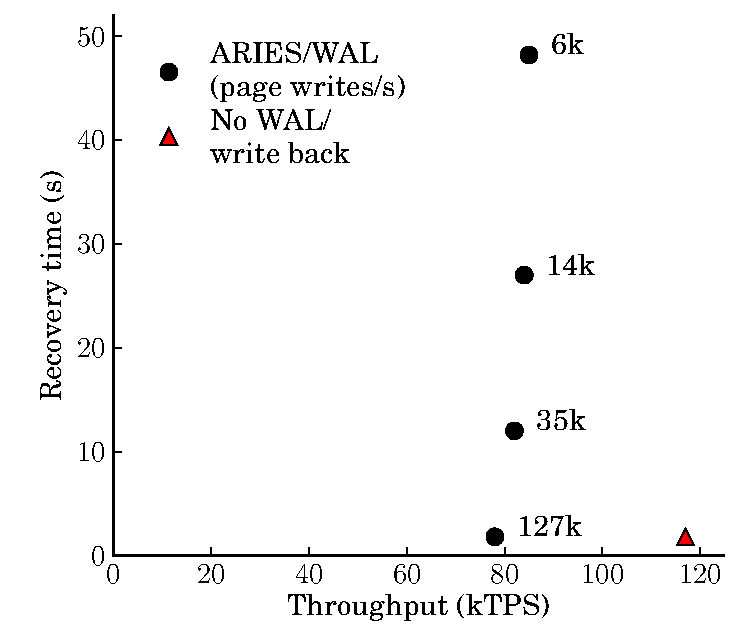
\includegraphics[width=.6\linewidth]{OLTP_design/TPCB_Recovery.pdf}
  \caption{\textbf{TPCB recovery latency vs throughput.} Increasing page flush rate reduces recovery latency.  Removing WAL entirely improves throughput by 50\%.}
  \label{fig::Recovery}
\end{figure}


The ARIES/WAL points (black circles) in the Figure show forward-processing throughput (horizontal axis) and recovery time (vertical axis) as a function of device write throughput (annotated alongside each point).
As database throughput can greatly outpace existing storage devices (this configuration requires 6,000 page writes/s to bound recovery at maximum transaction throughput; measured disk and flash devices provide only 190 and 2,500 page writes/s, respectively) I model recovery performance under faster NVRAM using a RAM disk for log and store while limiting the page flush rate.
As intuition would suggest, greater write bandwidth enables more aggressive flushing, minimizing the number of dirtied pages in the buffer cache at the time of failure, reducing recovery time.
With enough write bandwidth (in this case, 127,000 flushes/s, or 0.97 GB/s random writes for 8KB pages) the database recovers near-instantly, but forward-processing performance remains compute bound.
Achieving such throughput today requires large, expensive disk arrays or enterprise flash storage devices; future NVRAM devices might enable similar performance on commodity systems.

NVRAM opens up even more exciting opportunities for recovery management if we consider re-architecting database software.
The Figure shows this additional potential with a design point (red triangle) that removes WAL and asynchronous page flushing---optimizations primarily designed to hide disk latency.
Throughput improves due to three effects: (1) threads previously occupied by page and log flushers become available to serve additional transactions, (2) asynchronous page flushing, which interferes with transactions as both flusher and transaction threads latch frequently accessed pages, is removed, and (3) transactions no longer insert WAL log entries, reducing the transaction code path.
In aggregate these simplifications amount to a 50\% throughput increase over ARIES's best possible NVRAM performance.
The key take-away is that database optimizations long used for disk only hinder performance with faster devices.
In this chapter, I investigate how to redesign durable storage and recovery management for OLTP to take advantage of the low latency and byte-addressability of NVRAM.

NVRAMs, however, are not without their limitations.
Se\-veral candidate NVRAM technologies exhibit larger read latency and significantly larger write latency compared to DRAM.
Additionally, whereas DRAM writes benefit from caching and typically are not on applications' critical paths, NVRAM writes must become persistent in a constrained order to ensure correct recovery.
I consider an NVRAM access model where correct ordering of persistent writes is enforced via \emph{persist barriers}, which stall until preceding NVRAM writes are complete; such persist barriers can introduce substantial delays when NVRAM writes are slow.

This chapter outlines an approach to architecting recovery management for transaction processing using NVRAM technologies
I discuss potential performance problems with using NVRAM and possible software architectures to address these problems.
Additionally, I propose an evaluation framework, involving memory trace analysis, code annotation, and precise timing models for OLTP running on existing hardware platforms.
Subsequent chapters will build on the designs and methodology presented here to determine when OLTP must be redesigned and what problems might remain.
